
When designing C++ applications, performance is usually a key factor. While using the language can go a long way in the scope of a single application, the proper high-level design is also essential to achieving optimal latency and throughput. Let's discuss a few crucial patterns and aspects.

\subsubsubsection{4.5.1\hspace{0.2cm}CQRS and event sourcing}

There are many ways to scale compute but scaling data access can be tricky. However, it's often necessary when your userbase grows. \textbf{Command-query responsibility segregation (CQRS)} is a pattern that can help here.


\hspace*{\fill} \\ %插入空行
\noindent
\textbf{Command-query responsibility segregation}

In traditional CRUD systems, both reads and writes are performed using the same data model and the data flows the same way. The titular segregation basically means to treat queries (reads) and commands (writes) in two separate ways.

Many applications have a strongly biased ratio of reads to writes – there's usually a lot more reading from the database than updating it in a typical app. This means making the reads as fast as possible can yield better performance: reads and writes can now be optimized and scaled separately. Other than that, introducing CQRS can help if many writes are competing with each other, or if a track of all the writes needs to be maintained, or if a set of your API users should have read-only access.

Having separate models for reads and writes can allow having different teams to work on both sides. The developers working on the read side of things don't need to have a deep understanding of the domain, which is required to perform updates properly. When they make a request, they get a \textbf{data transfer object (DTO)} from a thin read layer in just one simple call instead of going through the domain model.

If you're not aware of what a DTO is, think of returning item data from the database. If the caller asks for a list of items, you could provide them with an \textit{ItemOverview} object containing just the names and thumbnails of items. On the other hand, if they want items for a specific store, you could also provide a \textit{StoreItem} object containing a name, more pictures, a description, and a price. Both \textit{ItemOverview} and \textit{StoreItem} are DTOs, grabbing data from the same \textit{Item} objects in the database.

The read layer can reside either on top of the data storage used for writes, or it can be a different data storage that gets updated via events as you can see in the following figure:


\begin{center}
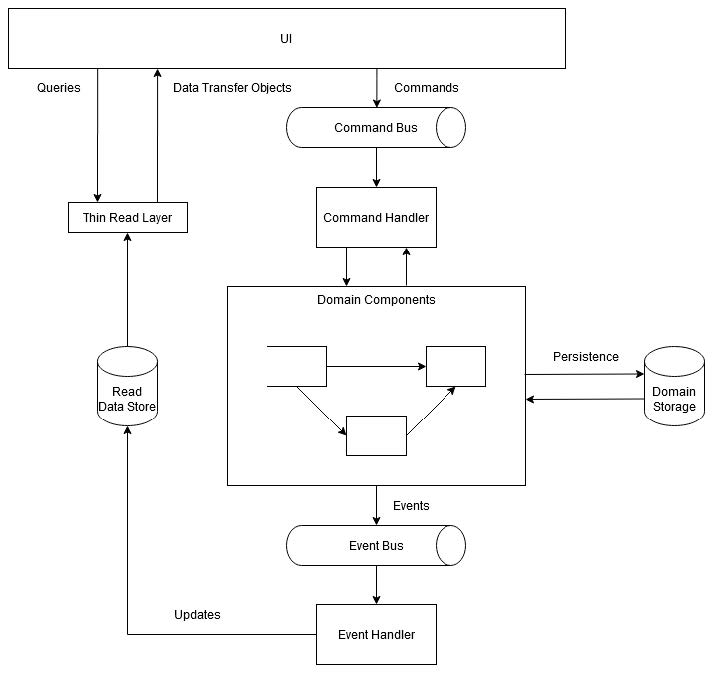
\includegraphics[width=0.9\textwidth]{content/2/chapter4/images/2.jpg}\\
Figure 4.2 – CQRS with event sourcing
\end{center}

Using the approach pictured here, you can create as many different commands as you like, each having its own handler. Usually, the commands are asynchronous and don't return any values to the caller. Each handler uses domain objects and persists the changes done. After doing that, events are published, which event handlers can use to update the storage used by read operations. Continuing our last example, item data queries would grab information from a database updated by events such as \textit{ItemAdded} or \textit{ItemPriceChanged}, which could be triggered by commands such as \textit{AddItem} or \textit{ModifyItem}.


Using CQRS allows us to have different data models for read and write operations. For instance, you can create stored procedures and materialized views to speed up reads. Using different types of storage (SQL and NoSQL) for the read and domain stores can also be beneficial: one efficient way to persist data is to use an Apache Cassandra cluster while using Elasticsearch is a great way to search through the stored data quickly.

Aside from the preceding pros, CQRS also has its cons. Due to the complexity it introduces, it's usually not a good fit for small or less requiring architectures. It's often useful to apply it only to the parts of your system where it would bring the biggest benefits. You should also notice that updating the read store after the domain store means that now we have eventual consistency instead of strong consistency.


\hspace*{\fill} \\ %插入空行
\noindent
\textbf{Command-query separation}

CQRS is actually based on a simpler idea introduced long ago in the Eiffel programming language (the same one that introduced contracts). \textbf{Command-query separation (CQS)} is a principle that devises to separate API calls into, well, commands and queries – just like in CQRS, but regardless of the scale. It plays really well with objective programming and imperative programming in general.

If your function's name starts with a \textit{has}, \textit{is}, \textit{can}, or a similar word, it should be just a query and not modify the underlying state or have any side effects. This brings two great benefits:


\begin{itemize}
\item 
\textbf{Much easier reasoning about the code}: It's clear that such functions are semantically just \textit{reads}, never \textit{writes}. This can make looking for a change of state much easier when debugging.

\item 
\textbf{Reduce heisenbugs}: If you have ever had to debug an error that manifested in a release build, but not in the debug one (or the other way around), you have dealt with a heisenbug. It's rarely something pleasurable. Many such errors can be caused by assert calls that modify the state. Following CQS eliminates such bugs.
\end{itemize}

Similarly to asserts, if you want to have contracts (pre- and post-conditions), it's super important to only use queries in them. Otherwise disabling some contract checks could also lead to heisenbugs, not to mention how counterintuitive it would be.

Let's now say a few more words about event sourcing.


\hspace*{\fill} \\ %插入空行
\noindent
\textbf{Event sourcing}

As introduced in Chapter 2, Architectural Styles, event sourcing means that instead of always storing the whole state of your application, possibly dealing with conflicts during updates, you can just store the changes that happened to your application's state. Using event sourcing can boost your app's performance by eliminating concurrent updates and allowing all interested parties to perform gradual changes to their state. Saving the history of the operations done (for example, market transactions) can allow easier debugging (by replaying them later) and auditing. This also brings more flexibility and extensibility to the table. Some domain models can get much simpler when event sourcing is introduced.

One cost of event sourcing is being eventually consistent. Another one is slowing down the startup of your application – unless you make periodic snapshots of the state or can use the read-only store as in CQRS, discussed in the previous section.

Okay, enough of CQRS and related patterns. Let's now move on to another hot topic when it comes to performance (no pun intended): caching.

\subsubsubsection{4.5.2\hspace{0.2cm}Caching}

Proper usage of caches can yield better performance, lower latency, reduce the server load (and thus, costs of running in the cloud), and help with scalability concerns (fewer servers required) – what's not to like?

\begin{tcolorbox}[colback=blue!5!white,colframe=blue!75!black, title=Note]
\hspace*{0.7cm}If you're here for tips on CPU caches, you can find them in \textit{Chapter 11, Performance}.

\end{tcolorbox}

Caching is a big topic, so we'll only cover a few aspects of it here.

Caching works by simply storing the data that is read most often in non-persistent storage with fast access times. There are many different types of caches: 

\begin{itemize}
\item 
\textbf{Client-side caches}: For storing data specifically for a given customer, often placed on the client's machine or browser.


\item 
\textbf{Web server caches}: For speeding up reading from web pages, for instance, through HTTP accelerators such as Varnish that can cache the web server responses.

\item
\textbf{Database caches}: Many database engines have built-in, tunable caching.

\item
\textbf{Application caches}: For speeding up your application, which can now read data from a cache instead of reaching out to its database.


\item
\textbf{CDNs can be treated as caches too}: For serving content from a location close to the user in order to reduce latency.

\end{itemize}

Some types of caches can be replicated or deployed in clusters to provide performance at scale. An alternative can also be to shard them: similarly to as you would shard databases, you can use different instances of your caches for distinct parts of your data.

Let's now go through the different approaches to updating the data in the cache. After all, no one likes to be served stale data.


\hspace*{\fill} \\ %插入空行
\noindent
\textbf{Updating caches}

There are a few approaches to keeping the cached data fresh. Whether it's you who decided how to update cached items or another company, it's worth knowing them. In this section, we'll discuss their pros and cons.


\hspace*{\fill} \\ %插入空行
\noindent
\textit{Write-through approach}

If you require strong consistency, synchronously updating both the database and the cache is the valid approach for you. This approach protects you from data loss: if data became visible to a user, it means it is already written to the database. A downside of write-through caches is that the latency to perform the update is bigger than in other approaches.

\hspace*{\fill} \\ %插入空行
\noindent
\textit{Write-behind approach}

An alternative approach, also known as write-back, is to provide the user with just access to the cache. When the user performs an update, the cache will then queue the incoming update, which will then be asynchronously executed, thus updating the database. The obvious downside here is that if something goes wrong, the data can never be written. It's also not as easy to implement as the other approaches. The upside, however, is the lowest latency as seen by the user.


\hspace*{\fill} \\ %插入空行
\noindent
\textit{Cache-aside}

This last approach, also called \textbf{lazy loading}, is about filling the cache on-demand. In this case, data access looks as follows:


\begin{enumerate}
\item 
A call to the cache is made to check whether the value is already there. If so, just return it.

\item 
Reach the main data store or service that provides the value.

\item
Store the value in the cache and return it to the user.

\end{enumerate}

This type of caching is often done using Memcached or Redis. It can be really fast and efficient – the cache only contains data that was requested.

However, if data that is not in the cache is often requested, the preceding three calls can increase the latency noticeably. To mitigate this for cache restarts, the cache can be primed (initialized) with selected data from the persistent store.

The items in the cache can also become stale, so it's best to set a time-to-live for each entry. If the data is to be updated, it can happen in a write-through manner by removing the record from the cache and updating it in the database. Take care when using multi-level caches with just a time-based update policy (for instance, as in DNS caches). This may lead to using stale data for long periods of time.

We've discussed the types of caches and strategies to update them, so that's enough about caches for now. Let's move on to a different aspect of providing scalable architectures.






